% ---------------------------------------------------------
\chapter{Methodology}
\label{chap:p_measurement}
% ---------------------------------------------------------

 Measurement of performance is an important aspect of all kinds of science. 
% performance measurement of java 
% performance term is explained in chap Background
% how does mesurement of performance work in general?
% Impact from OS and Hardware (CPU overclock, memory access, memory level)
% Sampling Strategies


\section{Test Environment}
\label{test_env}


\section{Case Studies}
\label{case_studies}

Eingrenzung auf Java software because, widespread, popular, often used, runs on billions of devices

% 3 Java projects 
% 3 different kinds of projects to depict variety
% Configurable, Workload of projects to manage execution time and to validate results of projects with different workloads
% different configuration space 
% different ammount of configuration options
% 
% Definition of configuration space for subject systems\cite{Han:2016:ESP:2961111.2962602}:
% collection of information with studying all artifacts that are publicly available to users including documents (e.g. user manuals and online help pages), configuration files, and source code. -> anoter reason for open sourece projects because else there were only provided configurations available 

% proveded performance tests for the case studies
% Configuration space definition(\cite{Han:2016:ESP:2961111.2962602}): they also described the configuration space not only by parameter, but also with hidden configuration options and system-specific configurations
% they also described the configuration space not only by parameter, but also with hidden configuration options and system-specific configurations
% -> This thesis: system configuration options are restricted to one system to be able to limit the overall configuration options
% configuration parameter cause 78%-92% of configuration-related performance bugs
% for this thesis we do not investigate 8%-17% of system-level configuration bugs

\subsection{Catena}

 Project description
% Project size in Classes and Functions
% Project properties (SPL Model)
% Features explained
% Workload

\subsection{H2}

Project description
% Project size in Classes and Functions
% Project properties (SPL Model)
% Features explained
% Workload

\subsection{Sunflow}

Project description
% Project size in Classes and Functions
% Project properties (SPL Model)
% Features explained
% Workload

\section{Overall Process}
\label{overall_process}

\begin{figure}
  \centering
  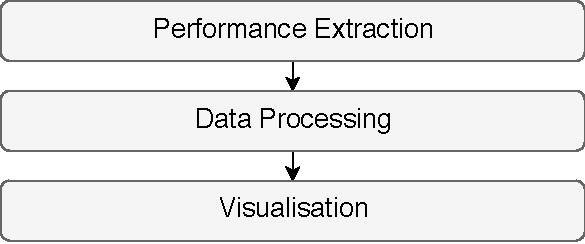
\includegraphics[width=0.7\textwidth]{images/workflow_overview_0}
  \caption{Performance Analysis Workflow.}
  \label{big_picture_perf_anal_workflow}
\end{figure}

% Overview of the process
\todo{Some information from the following paragraph might be shifted to chap. \ref{chap:p_measurement}}
We divided our approach into three parts as seen in Figure~\ref{big_picture_perf_anal_workflow}. First, we extract the performance data from the subject systems we used (see section~\ref{perf_extr}). Therefore, we run them in our test environment, which we describe in section~\ref{test_env}. We execute each of them with different configurations and workloads. We sampled the space of all possible configuration as described in the next section (section~\ref{perf_measure_sampling}) During execution, they were profiled to extract the performance of each method of the projects which was executed (we surveyed available performance monitoring tools in section~\ref{monitoring_tools}). In the second step, which is described more precisely in section~\ref{data_prozessing}, we process the collected data. We also trained a regression model that aims on predicting the performance of each method depending on given configurations. The last step of our approach includes visualizations of performance data (described in section~\ref{visualisation}). We designed an Eclipse plugin to visualize performance hot spots through the \ac{IDE} directly in the source code. Additionally, we used a graph-based visualisation to given an overview of the influence if configuration options on the performance of software systems.


\subsection{Performance extraction}
\label{perf_extr}

\begin{figure}
  \centering
  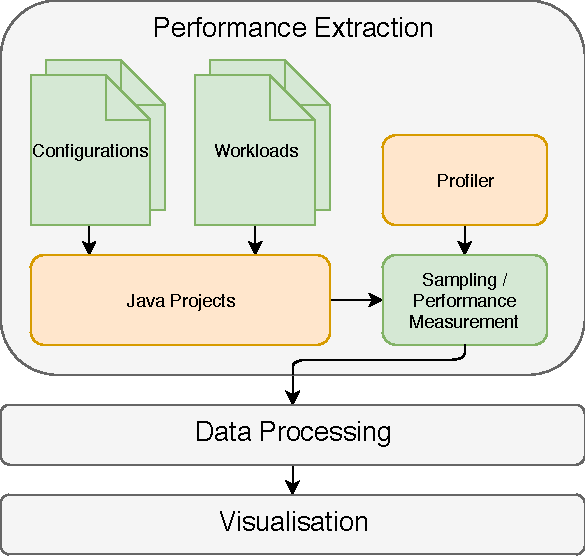
\includegraphics[width=0.7\textwidth]{images/workflow_perf_expanded}
  \caption{Performance Extraction Worklow.}
  \label{perf_extr_workflow}
\end{figure}


This section deals with performance extraction from configurable software systems. Figure \ref{perf_extr_workflow} shows our procedure. The orange parts of this diagram represent existing software and tools we used for this thesis, the green parts are results of our work. We choose three Java projects from GitHub as case studies. To be able to run software, it has to be initialize with parameters (configuration) and executed with a task (workload). Depending on the software, there are many different configurations to choose from. Also the number of different workloads depends on the software and the expected output. A general description of the projects, the space of possible configurations, and workloads was explained in section~\ref{case_studies}. Besides a configuration and workload, software needs an environment in which it can be executed. The environment can be defined by hardware, \ac{OS}, software and system settings. In order to measure performance during execution, we used the \ac{JIP} (section~\ref{perf_measure} compares different Java profiler). This profiler is able to measure the run time of each method during execution of the software. However, we have to deal with the influence of non-determinism that affect overall performance. Our measurements run on real hardware (test environment is described in section~\ref{test_env}) in a \ac{JRE} with other processes being executed in parallel. 

%Because software runs on real hardware, the measurements might be influenced by a measurement bias. Hence, we want to find out if and to which degree the environment has an influence on performance. We also trained a regression model that aims on predicting the performance of each method depending on given configurations. An introduction to linear regression and an overview of the tools we used for modelling can be found in section~\ref{lin_reg}. 

\subsubsection{System Influences}

separate machine
Multithreading
Only needed software installed
5 seconds delay between individual measurements

%Java specific performance measurement concerns~\ref{perf_measure}

%\subsection{Monitoring/Profiling}
%pitfalls
%strategies 
%solutions
%expected outcome
%A detailed analysis of available profiling tools is provided in section~\ref{perf_measure}. 


%Extracting performance of software. 
%Software is configurable.
%Identification of configuration options.
%Profile them with some workload.

%Performance of software is defined as described in~\ref{def:perf2}.

%Sources of non-determinism whole measuring performance.
%Environment in which software is executed is defined by hardware, \ac{OS}, software and system settings.
%Processes and threading is also a matter if on multi core machine.
%Because we want to analyze Java projects we have to take care about \ac{JIT}, \ac{GC} and \ac{JVM}.

\subsubsection{Java Mesurement Influences}
\label{perf_measure}

Java specific impacts on program execution and how to overcome them
% Related paper 
% Garbage collector
% Java Byte code optimization


\subsection{Data Processing}
\label{data_prozessing}

\begin{figure}
  \centering
  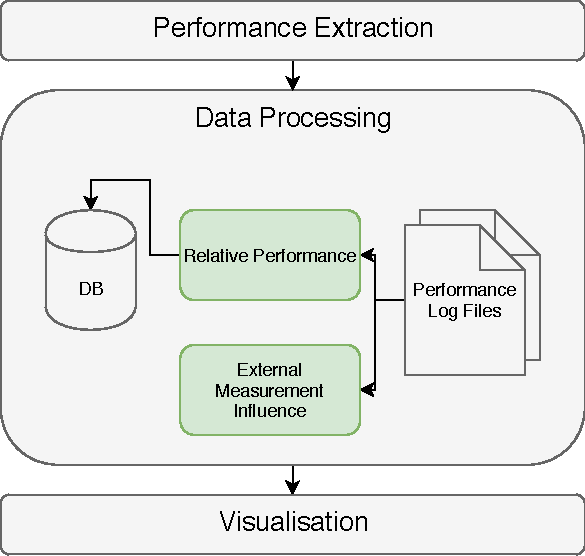
\includegraphics[width=0.7\textwidth]{images/workflow_data_expanded}
  \caption{Data Processing Worklow.}
  \label{perf_extr_workflow}
\end{figure}

\subsubsection{Relative Performance}

\subsubsection{Measurement Influence}


\subsection{Data Visualisation}
\label{visualisation}

\begin{figure}
  \centering
  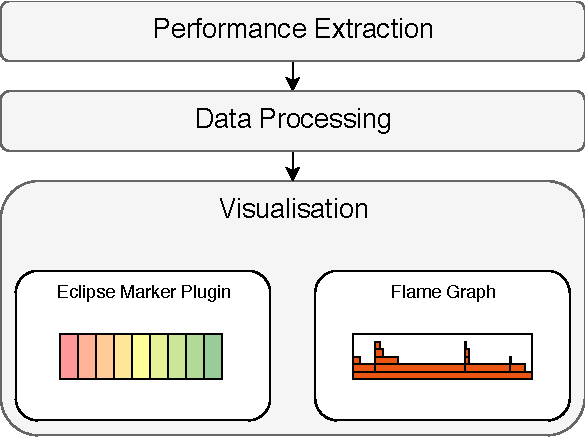
\includegraphics[width=0.7\textwidth]{images/workflow_visual_expanded}
  \caption{Visualisation Worklow.}
  \label{perf_extr_workflow}
\end{figure}

\subsubsection{Eclipse Plugin Data}

\subsubsection{Flame Graph Data}

